\subsection{M.PC.VP - Variazione del piano}

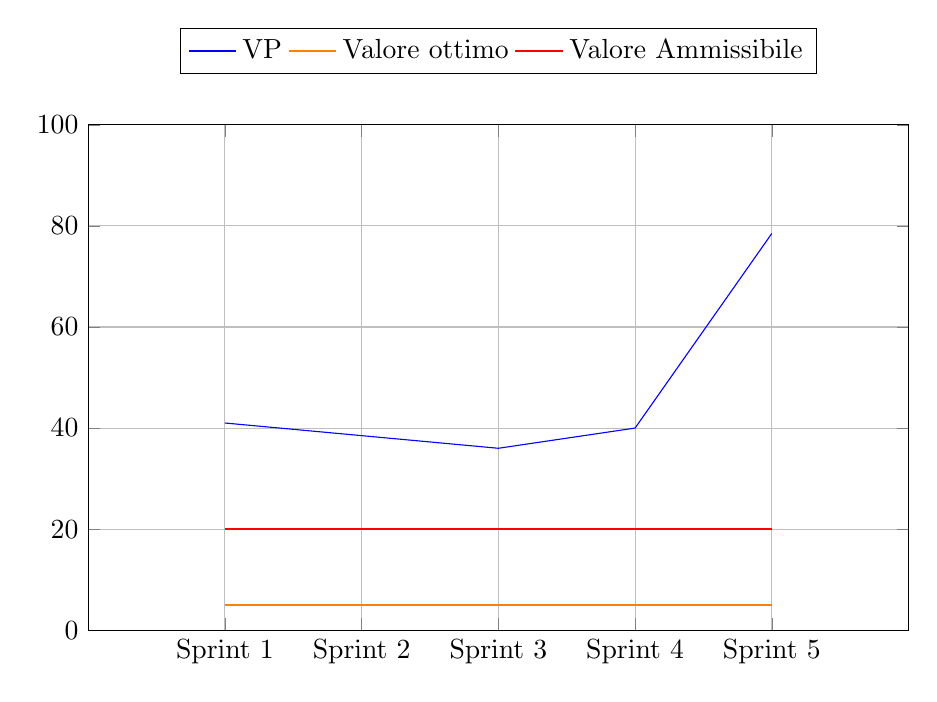
\begin{tikzpicture}
    \begin{axis}[
        width=12cm, height=8cm,
        ymin=0, ymax=100,
        xmin=0, xmax=6,
        xtick={1, 2, 3, 4, 5},
        xticklabels={Sprint 1, Sprint 2, Sprint 3, Sprint 4, Sprint 5},
        xlabel={},
        ylabel={},
        grid=major,
        scaled ticks=false,
        legend style={at={(0.5,1.1)}, anchor=south, legend columns=-1},
    ]
    \addplot[color=blue] coordinates {(1, 41) (2, 38.5) (3, 36) (4, 40) (5, 78.5)};
    \addlegendentry{VP}
    \addplot[orange, thick] coordinates {(1, 5) (5, 5)};
    \addlegendentry{Valore ottimo}
    \addplot[red, thick] coordinates {(1, 20) (5, 20)};
    \addlegendentry{Valore Ammissibile}
    \end{axis}
\end{tikzpicture}
\subsubsection{RTB}
Come si vede dal grafico la pianificazione è stata notevolmente errata, è stato pianificato un numero di attività 
eccessivo per ogni sprint portando a un numero elevato di attività non completate, per mancanza di tempo e di impegno da parte del gruppo.
Questo ha portato alla necessità di spostare in avanti la data per RTB inizialmente prevista per completare, durante gli ultimi sprint, le attività precedentemente pianificate.
  